\chapter{Introduction}
%\begin{enumerate}
%	\item We are interested in the decay, and want to describe what is happening.
%	\item Different levels which gives a continuum of 2+ state.
%	\item \isotope[8]{Li} har spin +2
%	\item We expect 2+ structure in \isotope[8]{Be}
%	\item There exists earlier measurements of \isotope[8]B	made in the AU group.
%	\item \isotope[8]B is the mirror core?? And has been measured very precisely.
%	\item Measure Li with same precision.
%	\item A beautiful spectrum from the alphas.
%	\item Look at a single alpha.
%	\item Look at coincidence.
%	\item Better to look at both and add, recoil will give widening.
%	\item read bataratjaa
%	\item We are interrested in beta alfa angles for \isotope[12]B
%	\item People have measured this angle precisely, because they where looking for deviations in the standard model.
%\end{enumerate}
%
%
%We want to examine the \be-delayed decay of \isotope[8]Li, which is an unstable isotope of Lithium. Lithium normally occurs stable as \isotope[6]Li and \isotope[7]Li, with the latter being the more abundant with 92.5\% of all atoms. The longest living radioactive lithium isotope is \isotope[8]Li, with a half-life of \SI{839}{ms} \note{ref}. 
%
%\li is an interesting atom, as it will decay into \isotope[8]Be, which is a constituent in the triple-alpha process in stellar astrophysics. \isotope[8]Be creates a bottleneck for the creation of heavier elements, as it is very short lived, and have a half-life of \SI{1e-16}{s}.
%
%\li will also decay into \ber at different energy levels, which will give a continuum of the 2+ state from \li. 
%
%The Sub-atomic group at Aarhus University has previously measured decay of the mirror nuclei, \isotope[8]B. Since there exists very precise measurement, we want to ¨obtain similar precise measurements of \li. 

\section{Motivation}
When Henri Becquerel first discovered radioactivity in the 1890's, a new branch of atomic physics was born, namely nuclear physics, which is the study of the atomic nuclei, their constituents and interactions. 
Over the years it has evolved quickly, first by the discovery of three different types of radiation by Curie and Rutherford, to the discovery of different nucleons, that the nucleus itself is made of. \\
\\
The technological advancements has made the study even more precise over the years, as the development of radioactive beams allow for the creation of specific short lived isotopes.
This technique is known as Isotope Separation On-Line (ISOL), which was first developed in 1951 for the Copenhagen Cyclotron. 
Now the technology is available in many parts of the world, such as the IGISOL facility at the University of Jyväskylä in Finland.
Another important advancement is the development of very precise detectors, such as the Double Sided Silicon Detector (DSSD), which allows for a very high energy and spacial resolution, which can give a detailed analysis of both coincidence and kinematics. \\
\\
This brings us onto the current experiment that i have analyzed in this thesis. At the IGISOL facility, the experiment I257 was carried out in august 2020. The objective of the experiment was to measure \be-decays from \li and \isotope[12]{B}, however, this thesis will only govern the \li decay. \\
The \be-\al\ angular correlation is previously shown with high precision to be nearly isotropic \cite{isotrop}. The study of the \be-\al\ correlation in \li will therefore serve as a good indicator for the \be-\al\ correlation in \isotope[12]{B}, as the same setup will be used for both experiment. \\
A former student has previously made an in depth analysis of the mirror nucleus \isotope[8]{B}, which can be used to compare the excitation energy of \ber. A comparison of the two is unfortunately out of scope for this thesis.


\section{Nuclear decays}
Lithium normally occurs stable as \isotope[6]Li and \isotope[7]Li, with the latter being the more abundant with 92.5\% of all atoms. The longest living radioactive lithium isotope is \isotope[8]Li, with a half-life of \SI{839}{ms} \note{ref}. 
When \li decays, it will do so under a \be-decay, immediately followed by the \al-\al\ breakup of an intermediate exited state in \ber, which has a half life of \SI{1e-16}{s}. \ber is a constituent in the triple-alpha process in stellar astrophysics, and creates a bottleneck for the creation of heavier elements, because of its very short lifespan.

%\li will also decay into \ber at different energy levels, which will give a continuum of the 2+ state from \li. 

\subsection{\be-decay}
Most light unstable nuclei will decay by either proton/neutron emission, or by a \be-decay. Isotopes that lie close to the valley of stability will not decay by proton/neutron emission, but from a \be-decay.
\\
A \be-decay is a weak interaction, which allows a quark in a proton or neutron to change flavor, by emitting a W boson. This leads to the creation of either an electron/antineutrino pair or a positron/neutrino pair, shown as:
\begin{align}
&\beta^+:\quad p\rightarrow n + e^+ + \nu_e\\
&\beta^-:\quad n\rightarrow p + e^- + \bar{\nu_e}.
\end{align}
Nuclei below the valley of stability will decay by $\beta^-$, while nuclei above decays by $\beta ^+$.

The energy for these decays are given by their Q-values, neglecting the very small neutrino mass and the binding energy of the electrons gives:
\begin{align}
&Q_{\beta^+} = \left[ m (\isotope[A][Z]{X}) - m(\isotope[A][Z-1]{X'})  		 \right] c^2\\
&Q_{\beta^-} = \left[ m (\isotope[A][Z]{X}) - m(\isotope[A][Z+1]{X'}) -2m_e  \right] c^2,
\end{align}
where $m$ is the mass of an atom with $Z$ protons and $A$ nucleons.
The Q-values indicates the mass difference between the initial and final product., which can be either excitation energy or kinetic energy. 

Not all \be-decays are allowed. If the spin is unchanged, it is a Fermi transition, and if it changes it is a Gamow-Teller transition. 
An allowed decay is a transition with the orbital angular moment $L = 0$, and forbidden transitions is $L > 0$.

The nuclear part of the \be-decay operator for an allowed decay is:
\begin{equation}
	\mathcal{O} (\beta^\pm) = g_V \sum_{A}^{j=1}\tau_\mp (j) + g_A \sum_{A}^{j=1}\sigma(j)\tau_\mp(j),
\end{equation}
where $g_V$ is weak vector coupling constant, $\tau_\mp$ is the isospin step operator, $g_A$ is the weak axial coupling constant and $\sigma$ is the Pauli spin matrices.
The first term corresponds to the Fermi operator, and the second term to the Gamow-Teller operator. 
This raises some selection rules, that dictate that for a Fermi decay, spin, isospin and parity must not be changed, and for a Gamow-Teller transitions, $\Delta J = 0, \pm1$, $\Delta T = 0, \pm 1$, and $\Delta \pi = 0$.

The selection rules then enforces that not every energy level is populated in \ber. 

\subsection{\al-decay}
\al-decay is another type of radioactive decay, where the nucleus emits an \al-particle, and thereby decays into a different nucleus with the atomic number reduced by two.  
It has a Q-value of:
\begin{equation}
Q_\alpha =  \left[ m (\isotope[A][Z]{X}) - m(\isotope[A-4][Z-2]{X'})  	- m_\alpha	 \right] c^2.
\end{equation}
Usually it is only elements heavier than nickel that can decay via this process, as the binding energy per nucleon decreases, and therefore becomes unstable towards spontaneous fission type processes. The only known exception to this rule is then \ber, which is the only light nuclei that decays by \al-decay. 

\section{Structure of $^8$Be}
\cref{fig:berStructure} shows the excitation spectrum for \ber, with values from \cite{TILLEY2004155}. The spin, parity and isospin are written as $J^\pi ; T$ for each level. 4 different states has been shown for \ber, where only the first excited state is the broad state at \SI{3.03}{MeV}. This state has conservation of spin and parity from \li and is the only state that is allowed for the decay of \li. Sittuated above is the broad state at \SI{11.35}{MeV}, which does not conserve spin. Above that is a \SI{16.626}{MeV} state, which conserves spin,parity and isospin, but lies energetically above \li, so we would not expect that to shown in the data. It is still a quite relevant state, as the mirror nucleus \isotope[8]{B} $(2^+; 1)$ lies just above the energy at \SI{17.979}{MeV}, and then has enough energy to populate this state, even though it is not very likely. Previous experiments made by the Aarhus subatomic group has examined the decay, and found only 5 counts populating this excitation level. But that should not show up when looking at the decay of \li.


\begin{figure}
	\centering
	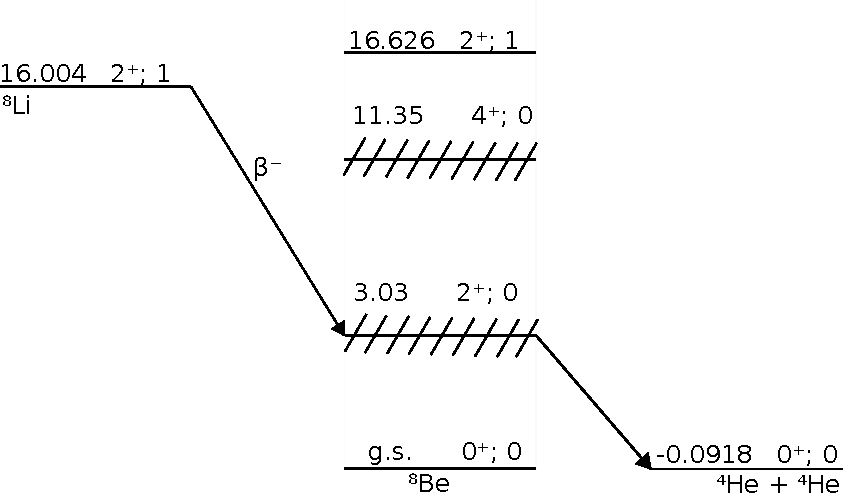
\includegraphics[width=\columnwidth]{../figures/DecayScheme.pdf}
	\caption{The decay scheme of \li, and some notable excitation energies of \ber. Each level is labeld with the energy above the \ber ground state in MeV. Spin parity and isospin is noted as $J^\pi; T$. All information is from \cite{TILLEY2004155}.}
	\label{fig:berStructure}
\end{figure}
